\documentclass{beamer}
\usepackage[spanish]{babel}
\selectlanguage{spanish}
\usepackage[utf8]{inputenc}
\usepackage{hyperref}
\usepackage{graphicx}
\usepackage{float}


\usetheme{Frankfurt}
\usecolortheme{whale}

\title{Ramas en Git}
\author{Emmanuel Arias \href{mailto:emmanuelarias30@gmail.com}{emmanuelarias30@gmail.com}}
\date{}
\begin{document}
\begin{frame}[plain]
    \maketitle
\end{frame}

\begin{frame}{Ramificaciones}
	\begin{itemize}
		 \item Cualquier sistema de control de versiones moderno tiene algún mecanismo para soportar el uso de ramas.
		 \item Cuando creamos un proyecto y nos mantenemos en la rama principal (master o main según cómo lo hemos creado) podemos seguir trabajando en la rama principal pero siempre vamos a necesitar realizar una copia del código para trabajar con esta.
		\item Muchos resaltan que uno de los puntos más fuertes de Git es su sistema de ramificaciones y lo cierto es que esto le hace resaltar sobre los otros sistemas de control de versiones. 
		\item Git maneja las ramas muy rápido haciendo que la operación de ramificación sea casi instantánea.
	\end{itemize}
\end{frame}

\begin{frame}{Ramas}
\begin{figure}
	\centering
	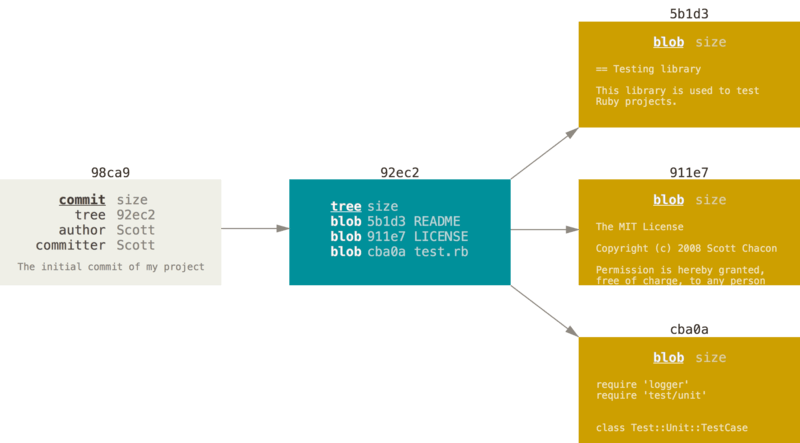
\includegraphics[width=1\linewidth]{img/commit-and-tree}
	\label{fig:commit-and-tree}
\end{figure}
\end{frame}

\begin{frame}{Ramas}
\begin{figure}
	\centering
	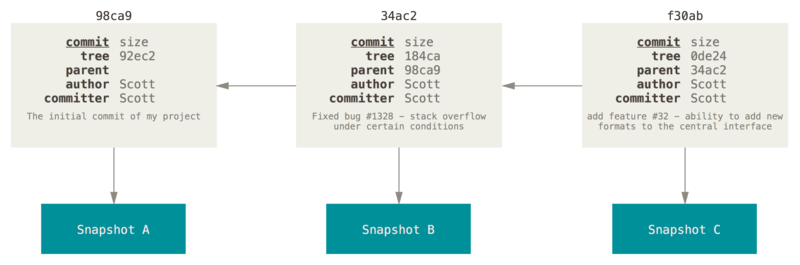
\includegraphics[width=1\linewidth]{img/2}
	\label{fig:2}
\end{figure}
\end{frame}

\begin{frame}{Ramas}
\begin{figure}
	\centering
	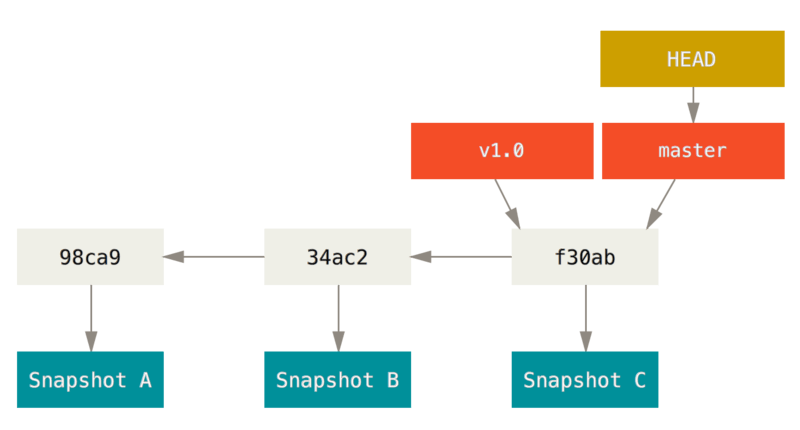
\includegraphics[width=1\linewidth]{img/3}
	\label{fig:3}
\end{figure}
\end{frame}

\begin{frame}{Ramas}
\begin{figure}
	\centering
	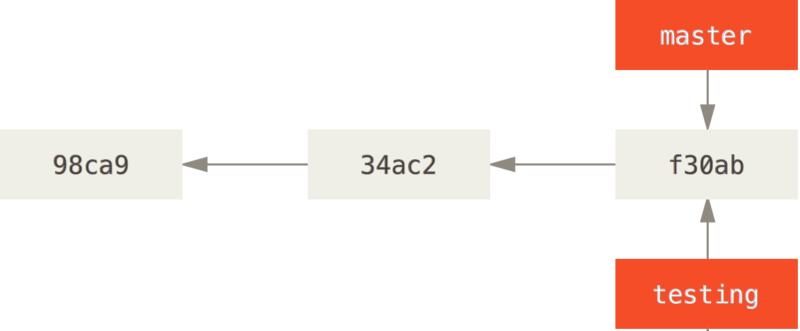
\includegraphics[width=1\linewidth]{img/4}
	\label{fig:4}
\end{figure}
\end{frame}

\begin{frame}{Ramas}
\begin{figure}
	\centering
	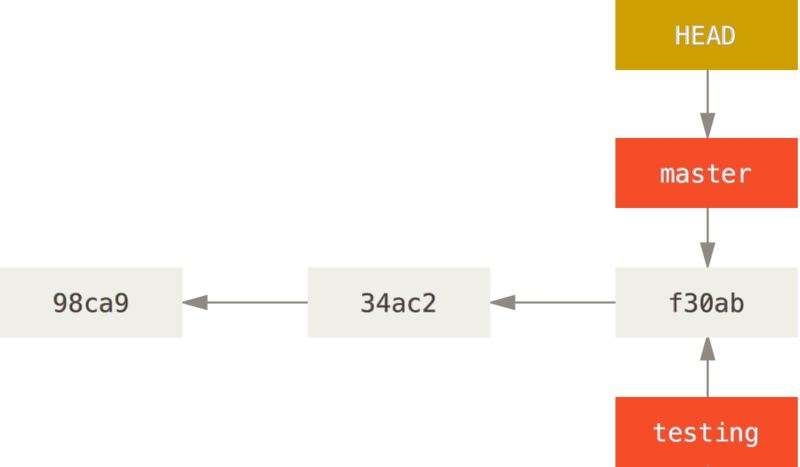
\includegraphics[width=1\linewidth]{img/5}
	\label{fig:5}
\end{figure}	
\end{frame}

\begin{frame}{Ramas}	
\begin{figure}
	\centering
	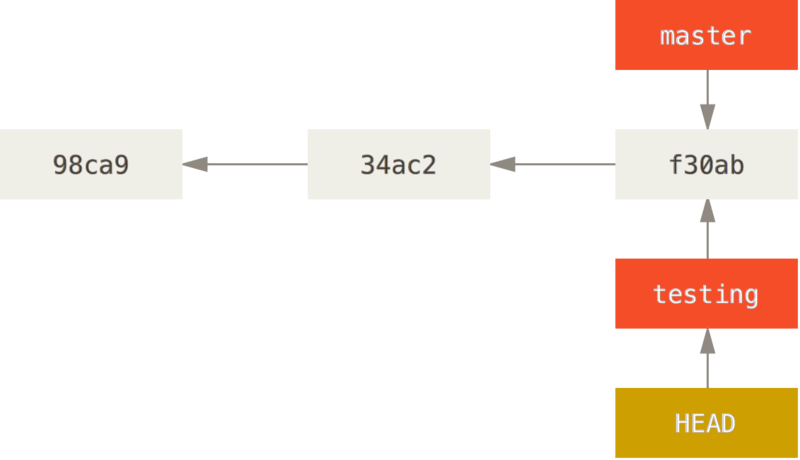
\includegraphics[width=1\linewidth]{img/5.1}
	\label{fig:5_1}
\end{figure}
\end{frame}

\begin{frame}{Ramas}
\begin{figure}
	\centering
	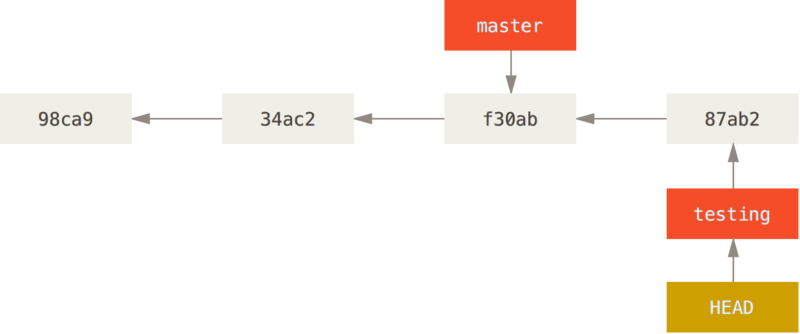
\includegraphics[width=1\linewidth]{img/6}
	\label{fig:6}
\end{figure}
\end{frame}

\begin{frame}{Ramas}
\begin{figure}
	\centering
	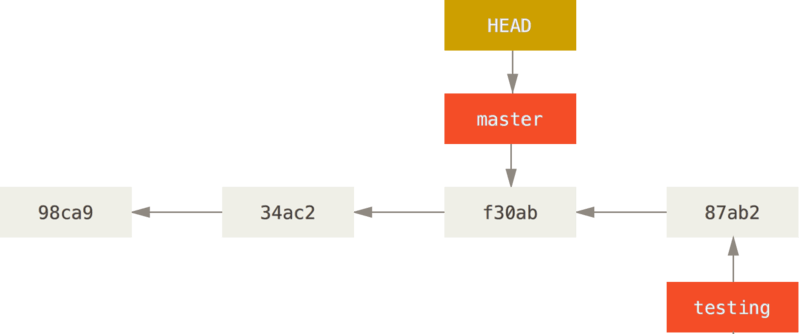
\includegraphics[width=1\linewidth]{img/7}
	\label{fig:7}
\end{figure}
\end{frame}

\begin{frame}{Ramas}
\begin{figure}
	\centering
	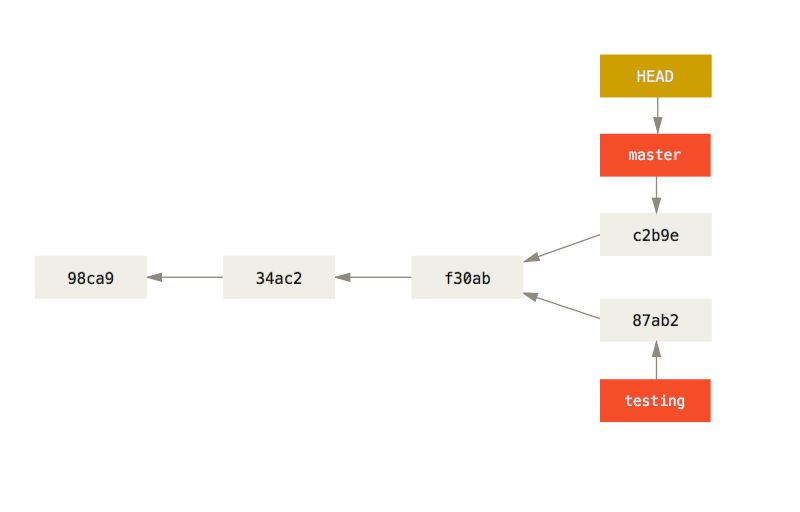
\includegraphics[width=1\linewidth]{img/8}
	\label{fig:8}
\end{figure}
\end{frame}

\end{document}
